\chapter{Simulator}
\label{chap:sim}

\begin{figure}
	\centering
	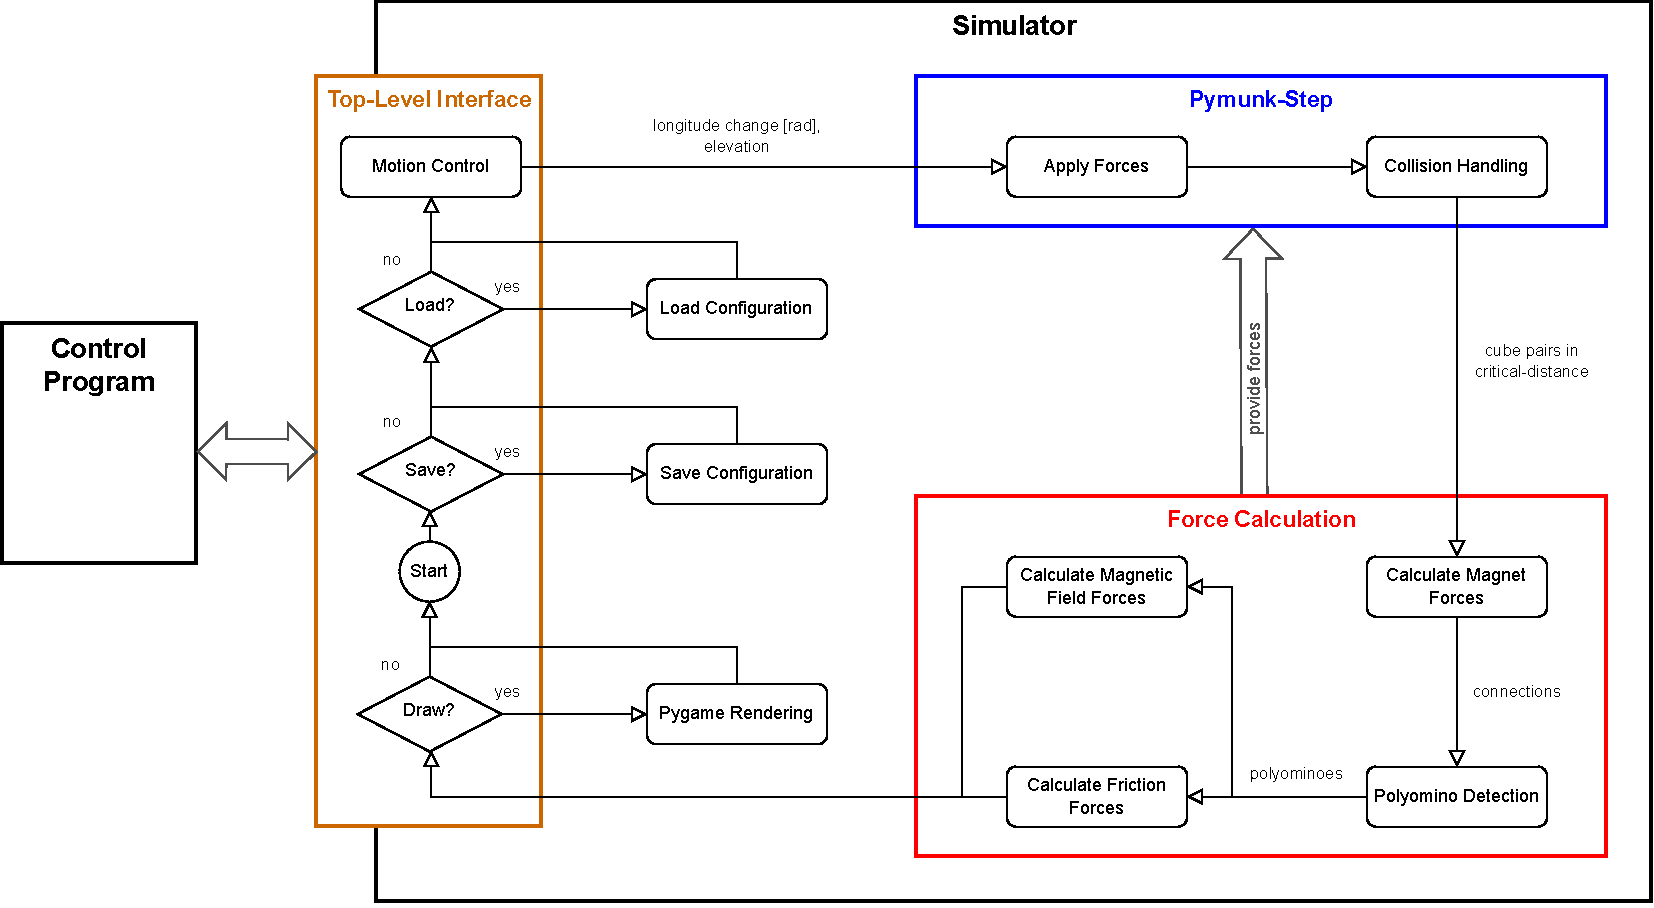
\includegraphics[width=1\textwidth]{figures/simulator_controlflow.pdf}
	\caption[Control flow of the simulator]{long caption...}
	\label{fig:simulator}
\end{figure}

% environmenmt python.  pymunk for simulating pygame for visualizing
% running headless only limited by computation time by space updating

% controlflow uml diagram flow-chart
% plot of time use for simulation


\section{Motion Control}

% rotaion linear ramp
% step sequence for motions
% handling elevation in 2D with friction
% waiting on motions to finish

\section{Configurations}

% what configuration consists of.
% cube info, poly info.
% polycollection functions as set and lists for polys
% everything hashable
% loading saving configs 

\section{Collision Handling}

% pymunks colison detection for cubes and walls -> Bounding volume hirachie
% used to determine range for magnetic forces

\section{Magnets}

% pull cubes together
% provide equation
% plot for magnetic attraction based on distance
% hold cubes together -> polyomino detection
% wich magnetic pairs to choose
% minDist, minDists, all

\section{Magnetic Field}

% applied to top bottom each indivial cube
% as long as orientation doenst match
% the bigger the poly the longer rotations actually take 
% adding zero updates to motion so that motion finishes when polys oriented


\section{Friction}

% force to let poly rotate around pivot point
% splitt friction on cubes on pivot edge
% nominal friction to prevent breaking


